
%(BEGIN_QUESTION)
% Copyright 2010, Tony R. Kuphaldt, released under the Creative Commons Attribution License (v 1.0)
% This means you may do almost anything with this work of mine, so long as you give me proper credit

A well-type manometer is used to measure the pressure generated by a Pitot tube sensing air speed.  The manometer already has a linear scale reading in centimeters water column, but you know the relationship between air speed and Pitot tube pressure is not linear:

$$\includegraphics[width=15.5cm]{i01404x01.eps}$$

You are told this Pitot tube generates 12.1 centimeters of static pressure at an air speed of 100 MPH.  Calculate the points along the centimeter scale corresponding to the following air speeds:

\begin{itemize}
\item{} 0 MPH = \underbar{\hskip 50pt} cm
\vskip 10pt
\item{} 20 MPH = \underbar{\hskip 50pt} cm
\vskip 10pt
\item{} 40 MPH = \underbar{\hskip 50pt} cm
\vskip 10pt
\item{} 60 MPH = \underbar{\hskip 50pt} cm
\vskip 10pt
\item{} 80 MPH = \underbar{\hskip 50pt} cm
\end{itemize}

\underbar{file i01404}
%(END_QUESTION)





%(BEGIN_ANSWER)

\begin{itemize}
\item{} 0 MPH = \underbar{\bf 0} cm
\vskip 10pt
\item{} 20 MPH = \underbar{\bf 0.484} cm
\vskip 10pt
\item{} 40 MPH = \underbar{\bf 1.936} cm
\vskip 10pt
\item{} 60 MPH = \underbar{\bf 4.356} cm
\vskip 10pt
\item{} 80 MPH = \underbar{\bf 7.744} cm
\end{itemize}

%(END_ANSWER)





%(BEGIN_NOTES)

{\bf This question is intended for exams only and not worksheets!}.

%(END_NOTES)

